\section{Results}
\label{sec:results}

\begin{figure}[!htbp]
\centering
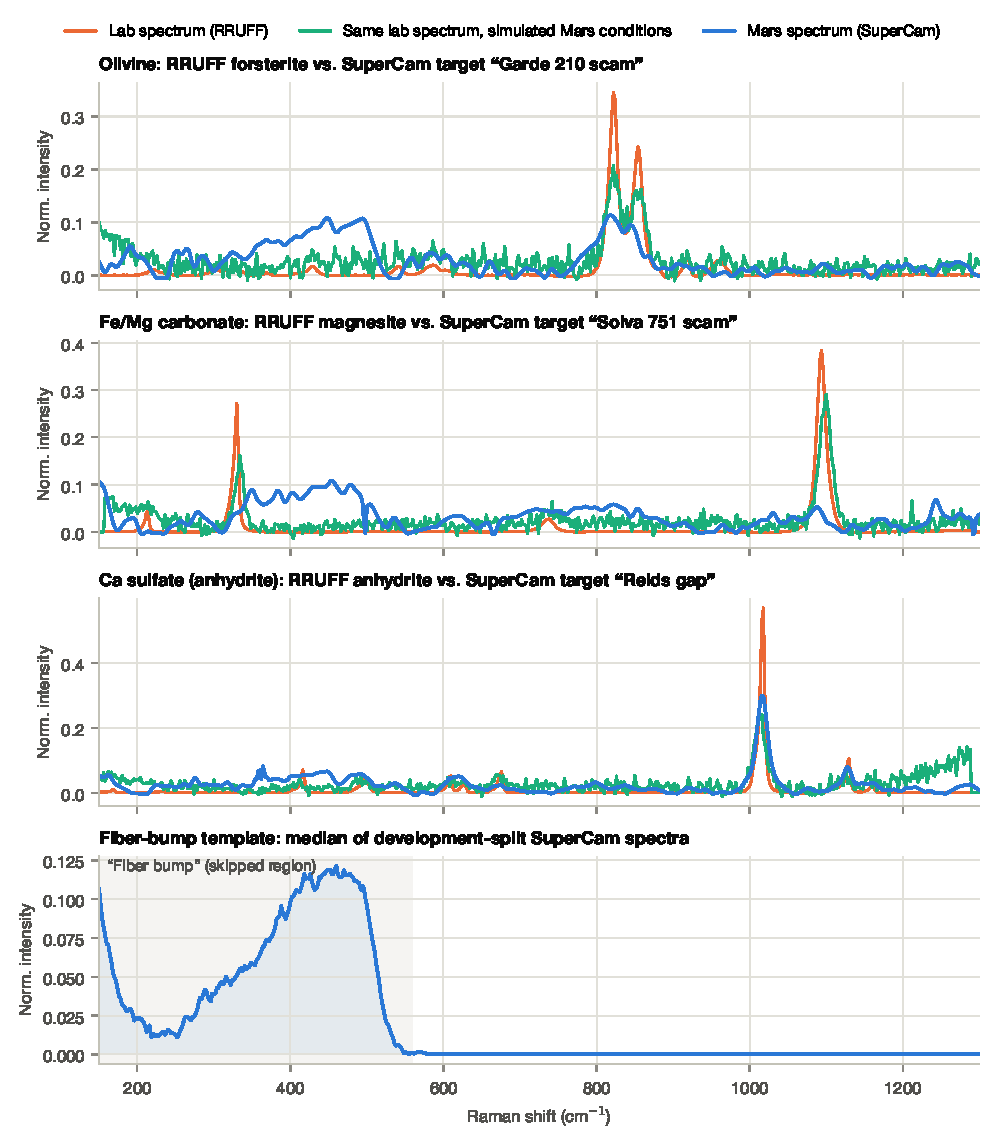
\includegraphics[width=0.82\linewidth]{figures/fig1_domain_gap.pdf}
\caption{\textbf{The lab-to-Mars gap.} Top three panels: a SuperCam spectrum (blue) for each of the three most common mineral groups, the matching RRUFF lab spectrum (orange), and the same lab spectrum after our simulated-Mars degradation (green). SuperCam peaks are broader and weaker relative to the background. Bottom: the median of the development-split SuperCam spectra, showing the broad ``fiber bump'' below about 560\,cm$^{-1}$ (shaded) that appears in most spectra whatever the mineral.}
\label{fig:gap}
\end{figure}

\subsection{In the lab, ``Shazam for minerals'' works}
On held-out lab samples, every method finds the right mineral group almost all the time: library search reaches \labGrpCleanCosineOpen{} group accuracy and \labSpCleanCosineOpen{} species accuracy across \nLabTestSpecies{} species. When the held-out lab spectra are degraded with our simulated-Mars effects, library search slips gradually, to \labGrpTwoCosineOpen{} group accuracy at twice the training strength. The CNN trained on simulated-Mars spectra is the most robust to these degradations (\labGrpTwoCnnMarsifiedOpen{} at strength 2; Figure~\ref{fig:simreal}a). If lab tests were the whole story, simulated-Mars training would look like a clear success.

\subsection{On Mars, the open library fails}
The picture changes completely on real SuperCam spectra (Table~\ref{tab:main}, Figure~\ref{fig:bars}). When predictions may be any RRUFF mineral, library search gets only \accCosineOpen{} of test spectra right (\balCosineOpen{} balanced accuracy), and no method exceeds \balCnnMarsifiedArtifactOpen{} balanced accuracy. The reason is easy to see in the matches. For \fracOtherOpen{} of Mars test spectra, the best library match is a mineral that is not in any group the team reports. For \fracAmorphOpen{}, it is a glass, opal, or other amorphous phase, led by synthetic rare-earth glasses and Libyan Desert glass. These materials have broad, featureless bands that resemble SuperCam's fiber bump, which on average carries \energyBumpMars{} of a Mars spectrum's normalized signal, compared with \energyBumpLab{} for lab spectra. The best cosine similarity is also lower on Mars (median \simMars{}) than between lab samples (median \simLab{}).

\begin{table}[!htbp]
\centering
\caption{\textbf{Main results.} Lab: mineral-group accuracy on held-out RRUFF samples (clean, open library; most held-out lab species lie outside the nine Mars groups, so the lab column is the same model scored without the Mars restriction). Mars: plain accuracy and balanced accuracy (mean recall over the six primary groups) on the \nMarsEval{} SuperCam test spectra, with 95\% cluster-bootstrap intervals over rocks. CNN numbers are three-seed ensembles. Bold: best balanced accuracy in each setting.}
\label{tab:main}
\small
\begin{tabular}{lcccc}
\toprule
 & Lab (clean) & \multicolumn{3}{c}{Mars test} \\
\cmidrule(lr){2-2}\cmidrule(lr){3-5}
Method & Group acc. & Acc. & Bal.\ acc. & 95\% CI (bal.) \\
\midrule
\multicolumn{5}{l}{\emph{Open library}}\\
Library search & 98\% & 5\% & 19\% & 2\%--24\%\\
\quad + skip fiber bump & 96\% & 6\% & 17\% & 1\%--21\%\\
\quad + resolution-matched & 98\% & 5\% & 21\% & 1\%--25\%\\
\quad + resolution-matched + skip & 95\% & 12\% & 28\% & 6\%--36\%\\
CNN, lab spectra & 98\% & 6\% & 26\% & 0\%--30\%\\
\quad + skip fiber bump & 98\% & 2\% & 7\% & 0\%--9\%\\
CNN, simulated-Mars training & 98\% & 7\% & 27\% & 2\%--31\%\\
\quad + skip fiber bump & 97\% & 5\% & 16\% & 2\%--20\%\\
\quad + fiber-bump template & 98\% & 13\% & \textbf{32\%} & 5\%--39\%\\
\addlinespace
\multicolumn{5}{l}{\emph{Mars-candidate library}}\\
Library search & 98\% & 45\% & 60\% & 33\%--66\%\\
\quad + skip fiber bump & 96\% & 68\% & \textbf{72\%} & 51\%--79\%\\
\quad + resolution-matched & 98\% & 38\% & 56\% & 29\%--63\%\\
\quad + resolution-matched + skip & 95\% & 62\% & 66\% & 46\%--73\%\\
CNN, lab spectra & 98\% & 44\% & 63\% & 44\%--68\%\\
\quad + skip fiber bump & 98\% & 38\% & 55\% & 30\%--62\%\\
CNN, simulated-Mars training & 98\% & 22\% & 48\% & 25\%--54\%\\
\quad + skip fiber bump & 97\% & 24\% & 40\% & 14\%--46\%\\
\quad + fiber-bump template & 98\% & 44\% & 58\% & 38\%--66\%\\
\addlinespace
Always ``olivine'' & -- & 50\% & 18\% & -- \\
\bottomrule
\end{tabular}

\end{table}

\begin{figure}[!htbp]
\centering
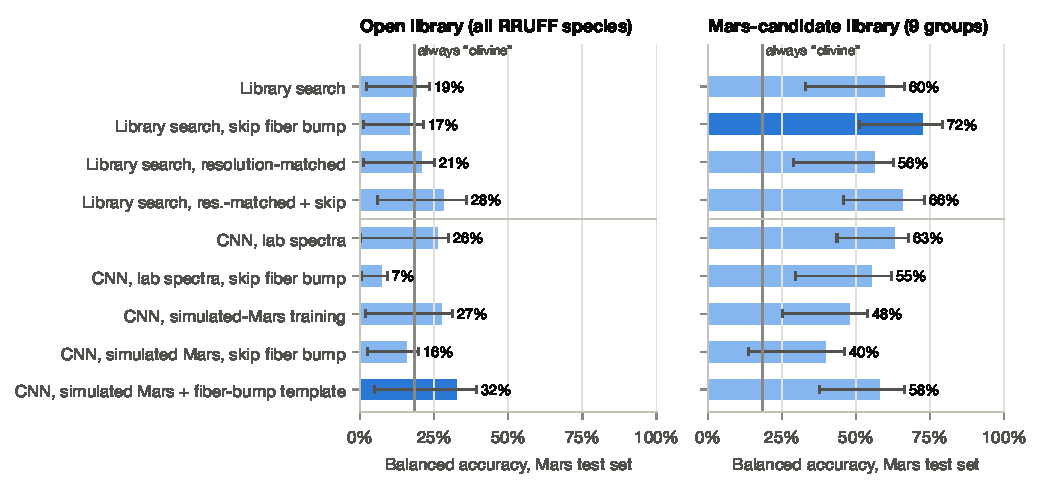
\includegraphics[width=\linewidth]{figures/fig2_mars_accuracy.pdf}
\caption{\textbf{Balanced accuracy on real SuperCam test spectra.} Left: predictions may be any RRUFF mineral. Right: predictions are restricted to the nine mineral groups reported in Jezero crater. Error bars are 95\% cluster-bootstrap intervals over rocks. The gray line is the trivial ``always olivine'' classifier. The darkest bar marks the best method in each panel.}
\label{fig:bars}
\end{figure}

\subsection{Prior knowledge and one simple fix recover most of the gap}
Restricting predictions to the Mars-candidate groups helps every method. Library search rises to \balCosineMars{} balanced accuracy (\accCosineMars{} accuracy). The single most effective change, however, is the simplest: skipping the fiber-bump region below 560\,cm$^{-1}$. With it, library search reaches \textbf{\balCosineWindowMars{}} balanced accuracy (95\% CI \balCICosineWindowMars{}) and \accCosineWindowMars{} accuracy, the highest score in this study. The gain over plain library search is \dWinVsCos{} percentage points (paired 95\% CI \dCIWinVsCos{}, $p=\pWinVsCos{}$). Its lead over the clean-lab CNN (\dWinVsCnn{} points, CI \dCIWinVsCnn{}, $p=\pWinVsCnn{}$) is not statistically significant with this test set, so we treat the two as roughly comparable, with library search ahead. The share of amorphous matches in the open setting falls from \fracAmorphOpen{} to \fracAmorphWindow{}. This choice is not an artifact of looking at the test set: on the development split, the skip variant is also the best library method (\devCosineWindow{} vs.\ \devCosine{} balanced accuracy) and beats the development-selected CNN (\devCnnClean{}). Per mineral, it identifies olivine in \recOlivineCosineWindowMars{} of cases and carbonate in \recCarbonateCosineWindowMars{} (Table~\ref{tab:recall}).

Matching the library to SuperCam's 12\,cm$^{-1}$ resolution, which one might expect to help, \emph{lowers} balanced accuracy both without the skip (\balCosineBroadenedMars{}) and with it (\balCosineBroadenedWindowMars{}). One possible explanation is that blurring makes many reference spectra look more alike, which costs more than the better peak-shape match gains.

\begin{table}[!htbp]
\centering
\caption{Recall per primary mineral group on the SuperCam test set (Mars-candidate setting).}
\label{tab:recall}
\small
\begin{tabular}{lcccccc}
\toprule
Method & Olivine & Carbonate & Sulfate & Pyroxene & Feldspar & Silica\\
 & ($n$=119) & ($n$=77) & ($n$=29) & ($n$=12) & ($n$=10) & ($n$=8)\\
\midrule
Library search & 36\% & 38\% & 79\% & 25\% & 80\% & 100\%\\
Library search, skip bump & 78\% & 58\% & 28\% & 100\% & 70\% & 100\%\\
Library search, res.-matched & 26\% & 34\% & 72\% & 25\% & 80\% & 100\%\\
Library search, res.-matched + skip & 68\% & 60\% & 24\% & 92\% & 50\% & 100\%\\
CNN, lab spectra & 29\% & 44\% & 72\% & 42\% & 90\% & 100\%\\
CNN, lab spectra, skip bump & 18\% & 48\% & 66\% & 50\% & 50\% & 100\%\\
CNN, simulated Mars & 5\% & 13\% & 79\% & 0\% & 90\% & 100\%\\
CNN, sim.\ Mars, skip bump & 21\% & 14\% & 34\% & 8\% & 60\% & 100\%\\
CNN, sim.\ Mars + template & 39\% & 38\% & 66\% & 17\% & 90\% & 100\%\\
\bottomrule
\end{tabular}

\end{table}

\subsection{Simulated-Mars training does not transfer to real Mars}
The CNN trained on clean lab spectra was selected on the development split. It reaches \balCnnCleanMars{} balanced accuracy on the test set (individual seeds: $\pm$\seedSdCnnCleanMars{} points standard deviation), close to plain library search but well below the skip variant. Our simulated-Mars training, which made the CNN the most robust model on degraded lab spectra, \emph{lowers} real-Mars balanced accuracy to \balCnnMarsifiedMars{}, a significant drop (\dCnnVsSim{} points for the clean-lab CNN, CI \dCICnnVsSim{}, $p=\pCnnVsSim{}$). Skipping the fiber bump does not rescue it (\balCnnMarsifiedWindowMars{}). Adding the fiber-bump template recovers part of the loss (\balCnnMarsifiedArtifactMars{}; \dTplVsSim{} points, CI \dCITplVsSim{}, not significant) and gives the best open-library score (\balCnnMarsifiedArtifactOpen{}), but it still does not beat the CNN trained on clean lab spectra. Figure~\ref{fig:simreal}b summarizes the mismatch: among our methods, accuracy under simulated Mars conditions does not predict accuracy on real Mars. If anything, the trend is negative.



\begin{figure}[!htbp]
\centering
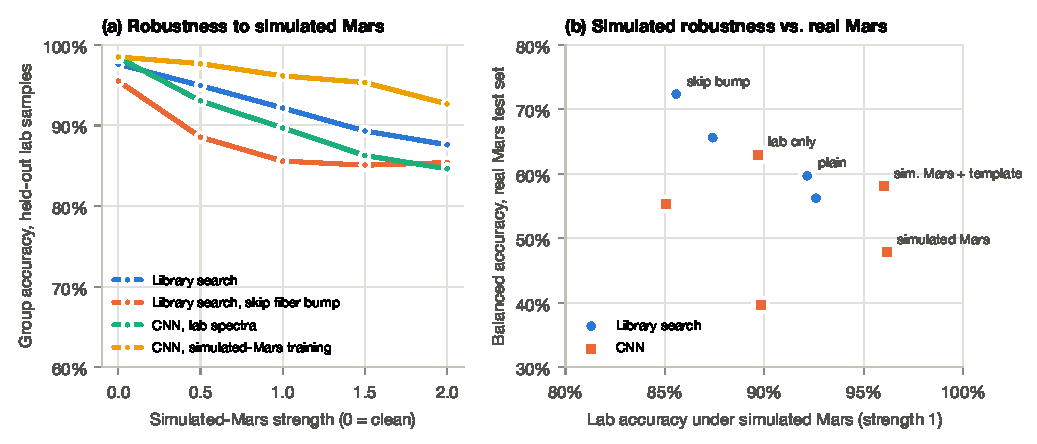
\includegraphics[width=\linewidth]{figures/fig3_sim_vs_real.pdf}
\caption{\textbf{Robustness to simulated Mars does not predict success on real Mars.} (a) Mineral-group accuracy on held-out lab spectra as the simulated-Mars degradation gets stronger (open-library setting). (b) For every method, lab accuracy under simulated Mars (strength 1) against balanced accuracy on the real SuperCam test set.}
\label{fig:simreal}
\end{figure}

\paragraph{Which simulated effect hurts?} To find out, we retrained the CNN with one simulated effect at a time (two seeds each; Figure~\ref{fig:single}). On the test set, \emph{every} single effect lowered balanced accuracy relative to no simulation (\seNoneTest{}): resolution blur \seResTest{}, calibration shift \seShiftTest{}, broad background \seBgTest{}, noise \seNoiseTest{}, and mineral mixing \seMixTest{}, the largest drop. All five together gave \seAllTest{}. Mixing was also the most harmful effect on the development split (\seMixDev{} vs.\ \seNoneDev{}). There, noise and background alone looked helpful (\seNoiseDev{} and \seBgDev{}), but the development split is small and the test set did not confirm this. One reading is that synthetic mixtures teach the network that a weak extra peak can be ignored, while on Mars weak peaks are often the signal itself.

\begin{figure}[!htbp]
\centering
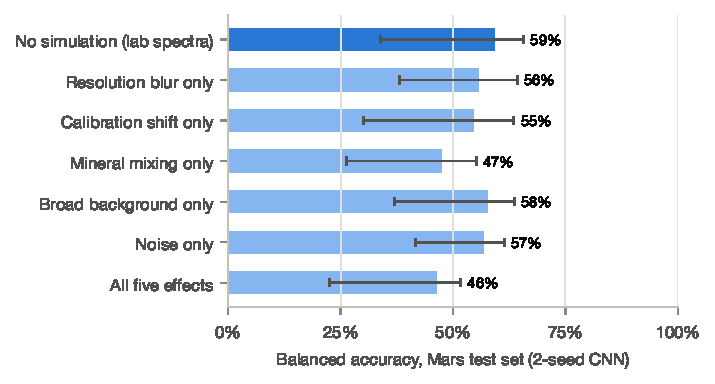
\includegraphics[width=0.7\linewidth]{figures/fig5_single_effects.pdf}
\caption{\textbf{One simulated effect at a time.} Balanced accuracy on the SuperCam test set (Mars-candidate setting) of CNNs trained with no simulation, with a single simulated-Mars effect, or with all five (two-seed ensembles; 95\% cluster-bootstrap intervals). The darkest bar marks training on clean lab spectra.}
\label{fig:single}
\end{figure}

\subsection{Where the errors are}
Figure~\ref{fig:confusion} shows the confusion patterns. Once the fiber bump is skipped, library search's remaining errors are mostly predictions of \emph{pyroxene}: for olivine, sulfate, and carbonate spectra alike, it is the most common wrong answer. Pyroxene's bands near 670 and 1010\,cm$^{-1}$ are broad on Mars and overlap anhydrite's main band at about 1017\,cm$^{-1}$. The clean-lab CNN instead tends to call olivine and carbonate spectra ``sulfate'' or ``feldspar''. Accuracy also follows the team's own confidence. For the skip variant, it is \confHighCW{} on high-confidence labels, \confMedCW{} on medium, and \confLowCW{} on low (\nConfHigh{}, \nConfMed{}, and \nConfLow{} spectra). The spectra that experts find hardest are hard for the algorithms too.

\begin{figure}[!htbp]
\centering
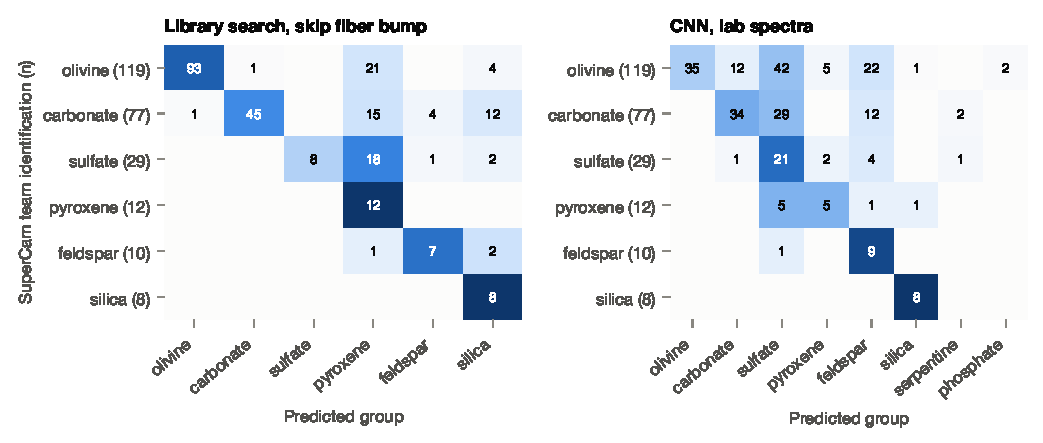
\includegraphics[width=\linewidth]{figures/fig4_confusion.pdf}
\caption{\textbf{Confusion matrices on the SuperCam test set} (Mars-candidate setting). Rows are the team's primary identification; a prediction that matches any group the team reported for that spectrum is counted on the diagonal. Cell color shows the fraction of the row.}
\label{fig:confusion}
\end{figure}
